


\documentclass[a4paper,11pt]{article} % ce document est un article sur une feuille A4, police taille 11
\usepackage[utf8]{inputenc}
\usepackage[T1]{fontenc} % compatible avec les accents
\usepackage{biblatex} %Imports biblatex package
\addbibresource{GAN video games.bib} %Import the bibliography file

\usepackage[french]{babel} % rédigé en français

\usepackage{graphicx} % gestion des images
\usepackage{array} % gestion des tableaux
\usepackage{csquotes} % gestion des guillemets
\usepackage{fourier} % utilise une autre police que celle par défaut (Computer Modern)

\title{Les réseaux antagonistes génératifs dans les jeux vidéos}
\author{Sarah Pirard}
\date{Décembre 2022}

\begin{document}

\maketitle

\section{Introduction}
Qu'est-ce qu'un réseau antagoniste génératif? Un réseau antagoniste génératif, également communément appelé "GAN" (generative adversarial network) est une classe d'algorithme qui permet de créer des images de synthèse à partir d'échantillons. Le principe est de mettre en opposition deux réseaux, en premier lieu le générateur, qui génère une image au discriminateur sur base d'un échantillon qui doit détecter si l'image est réelle ou si elle résulte de la création du générateur (\citeauthor{aggarwal_generative_2021}). Ce processus a été mis en place en 2014 par (\citeauthor{goodfellow_generative_2014}).Il en existe de nombreuses variantes à ce jour (Asimopoulos et al., 2022). Les GAN sont actuellement utilisés dans de nombreux domaines notamment dans l'imagerie médicale et le traitement d'image et de vidéo. Le domaine qui nous intéresse dans cet article est le domaine des jeux vidéos. (\citeauthor{noauthor_generative_2022})

\begin{figure}[h] % insère une figure ici (h = "here")
  \centering % centre la figure
  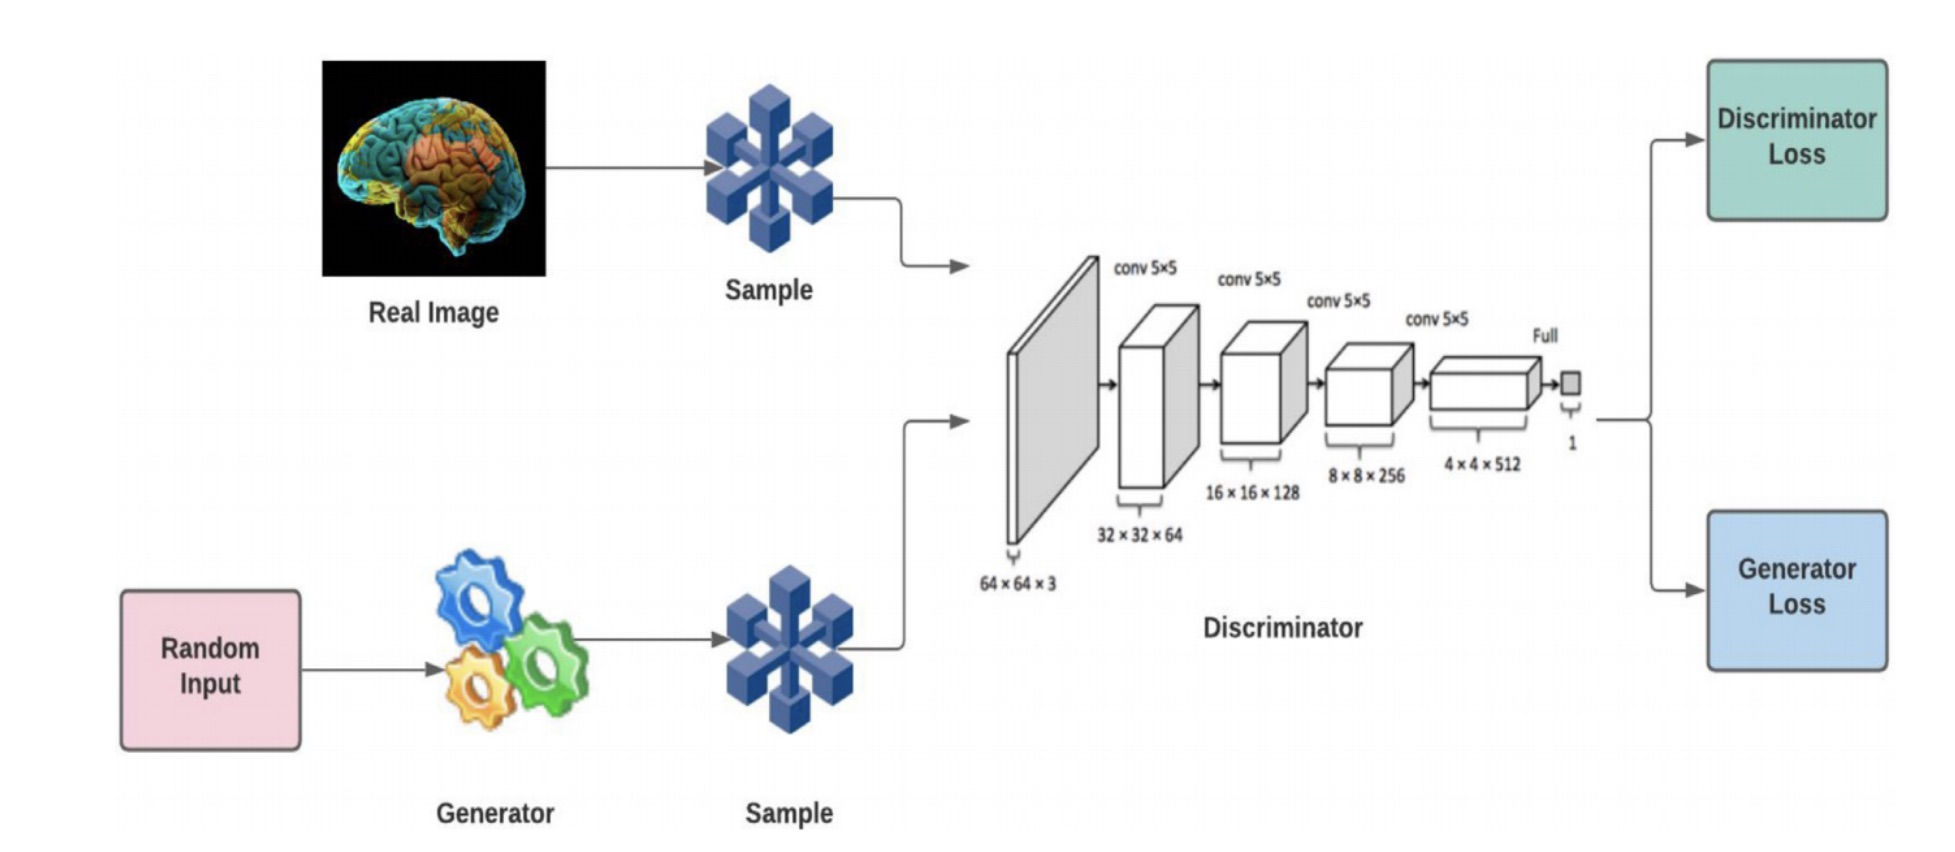
\includegraphics[scale=0.17]{GAN}
  \caption{fonctionnement d'un réseau antagoniste génératif} % nom de l'image
\end{figure}

\section{Quelles applications dans les jeux vidéos?}

\paragraph{
}
Les generative adversarial networks se sont montrés particulièrement efficaces en matière de PCG (Procedural Content Generation) dans le déploiement de nouveaux niveaux de jeux. Le PCG peut être utilisé pour générer des niveaux de jeu, des règles ou encore des textures pour les éléments graphiques. Il permet notamment de créer des mondes de jeux complexes en évitant de produire une surcharge de travail conséquente aux designers graphiques (Hendrikx et al, 2011). Cet approche a été récemment théorisée sous le nom de "Procedural Content Generation via Machine Learning" (PCGML) (Summerville et al.2018, Justesen et al. 2019; Guzdial et al 2018). Diverses systèmes d'architectures ont été utilisés en PCGML afin de générer du contenu de jeu .Les GAN ont gagné en popularité dans la production de jeux vidéos notamment grâce au fait qu'ils peuvent produire des environnements de jeux aléatoires sans nécessiter de supervision par un tiers. La méthode la plus accessible est basée sur une méthode de génération de nombres pseudo-aléatoire (PRNG). Les concepteurs utilisent ces modèles depuis les années quatre-vingts afin de générer des univers assez vastes, mais une démarche similaire est utilisée également pour concevoir les textures d'objets de jeu (\citeauthor{kumaran_generating_2020}). 

\paragraph{
}
Les GANs possèdent plusieurs caractéristiques clés qui permettent de les différencier dans la création de jeux vidéos des autres systèmes d'architecture. En premier lieu, ceux-ci permettent la modélisation de différents niveaux de jeux d'après une seule source. En appréhendant un modèle basé sur les GANs, il est possible de créer divers niveaux de jeux avec un gameplay similaire. Après avoir été joué, le niveau est ajouté au générateur comme exemple à confronter au discriminateur, ce qui permet au système de générer des niveaux de jeux continuellement. Une autre approche permet de se baser sur le gameplay d'un joueur pour générer progressivement des liveaux en utilisant des actions afin de produire un corpus (Shaker et al. 2015). 

\section{La synthèse des textures}

\paragraph{
}
Exprimé de manière théorique, une texture est la répétition d'un image d'une façon aléatoire. Le but dans la génération de textures lors de la création de jeux vidéos, et notamment la création du fond, est de capturer un échantillon de texture, dont le système permet la répétition de manière arbitraire. Deux méthodes différentes peuvent être utilisées. La première méthode consiste à replacer des échantillons visuels de textures afin de préserver ses propriétés visuelles. Cependant, cette méthode ne permet pas de produire une texture à proprement parler, mais simplement de réitérer un exemple encore et encore. La seconde méthode est de confronter des images statistiquement similaires afin de créer un fond avec une texture convaincante (\citeauthor{jetchev_texture_2017}).

\begin{figure}[h] % insère une figure ici (h = "here")
  \centering % centre la figure
  \includegraphics[scale=0.5]{texture}
  \caption{modélisation de la création de texture par réseau antagoniste génératif} % nom de l'image
\end{figure}



\begin{thebibliography}{}
\printbibliography

\end{thebibliography}

\end{document}
